\documentclass[border=5pt]{standalone}
\usepackage{tikz}
\usetikzlibrary{arrows.meta, positioning, decorations.pathreplacing, calc}
\usepackage{xcolor}

\definecolor{Garnet}{HTML}{73000A}
\definecolor{NinetyBlack}{HTML}{363636}
\definecolor{SeventyBlack}{HTML}{5C5C5C}
\definecolor{FiftyBlack}{HTML}{A2A2A2}
\definecolor{ThirtyBlack}{HTML}{C7C7C7}
\definecolor{TenBlack}{HTML}{ECECEC}
\definecolor{Atlantic}{HTML}{466A9F}
\definecolor{Rose}{HTML}{CC2E40}
\definecolor{Sandstorm}{HTML}{FFF2E3}

\tikzset{every node/.append style={rounded corners=0pt}}

\begin{document}
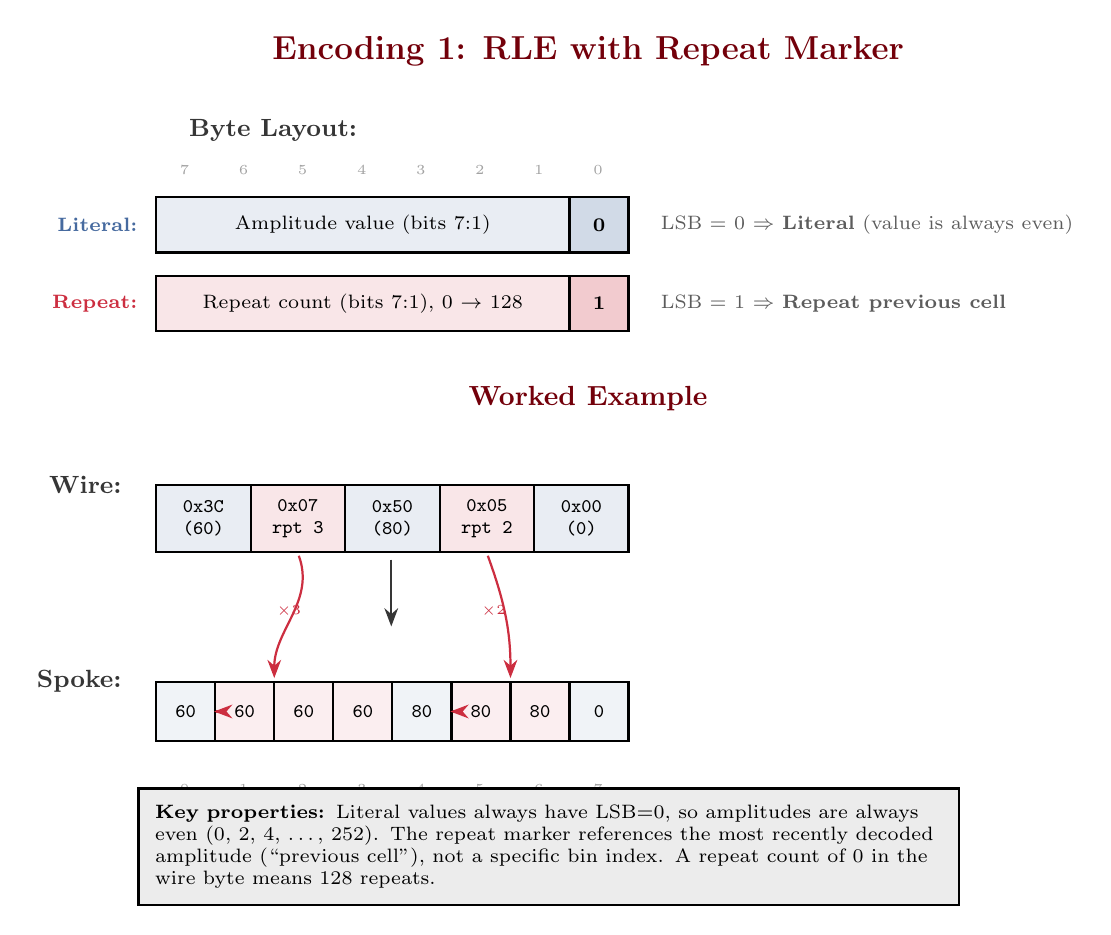
\begin{tikzpicture}[
    cell/.style={draw, thick, minimum width=1.2cm, minimum height=0.85cm, anchor=west, font=\ttfamily\scriptsize, align=center},
    scell/.style={draw, thick, minimum width=0.75cm, minimum height=0.75cm, anchor=west, font=\ttfamily\scriptsize, align=center},
    lbl/.style={font=\small\bfseries, color=NinetyBlack},
    annot/.style={font=\scriptsize, color=SeventyBlack},
]

\node[font=\bfseries\large, color=Garnet] at (5.5, 5.8) {Encoding 1: RLE with Repeat Marker};

% ── Bit layout explanation ──
\node[lbl] at (1.5, 4.8) {Byte Layout:};

% Literal byte
\node[draw, thick, fill=Atlantic!12, minimum width=5.25cm, minimum height=0.7cm, anchor=west, font=\scriptsize] at (0, 3.6) {Amplitude value (bits 7:1)};
\node[draw, thick, fill=Atlantic!25, minimum width=0.75cm, minimum height=0.7cm, anchor=west, font=\scriptsize\bfseries] at (5.25, 3.6) {0};
\node[annot, anchor=west] at (6.3, 3.6) {LSB = 0 $\Rightarrow$ \textbf{Literal} (value is always even)};
\node[font=\scriptsize\bfseries, color=Atlantic, anchor=east] at (-0.1, 3.6) {Literal:};

% Repeat byte
\node[draw, thick, fill=Rose!12, minimum width=5.25cm, minimum height=0.7cm, anchor=west, font=\scriptsize] at (0, 2.6) {Repeat count (bits 7:1), 0 $\rightarrow$ 128};
\node[draw, thick, fill=Rose!25, minimum width=0.75cm, minimum height=0.7cm, anchor=west, font=\scriptsize\bfseries] at (5.25, 2.6) {1};
\node[annot, anchor=west] at (6.3, 2.6) {LSB = 1 $\Rightarrow$ \textbf{Repeat previous cell}};
\node[font=\scriptsize\bfseries, color=Rose, anchor=east] at (-0.1, 2.6) {Repeat:};

% Bit position labels
\foreach \i/\v in {0/7, 1/6, 2/5, 3/4, 4/3, 5/2, 6/1, 7/0} {
    \node[font=\tiny, color=FiftyBlack] at (0.375 + \i*0.75, 4.3) {\v};
}

% ── Worked Example ──
\node[font=\bfseries, color=Garnet] at (5.5, 1.4) {Worked Example};

% Wire bytes
\node[lbl, anchor=east] at (-0.3, 0.3) {Wire:};
\node[cell, fill=Atlantic!12] (w0) at (0, -0.13) {\texttt{0x3C}\\(60)};
\node[cell, fill=Rose!12] (w1) at (1.2, -0.13) {\texttt{0x07}\\rpt 3};
\node[cell, fill=Atlantic!12] (w2) at (2.4, -0.13) {\texttt{0x50}\\(80)};
\node[cell, fill=Rose!12] (w3) at (3.6, -0.13) {\texttt{0x05}\\rpt 2};
\node[cell, fill=Atlantic!12] (w4) at (4.8, -0.13) {\texttt{0x00}\\(0)};

% Decode arrows
\draw[-{Stealth}, thick, NinetyBlack] (3.0, -0.65) -- (3.0, -1.5);

% Decoded spoke
\node[lbl, anchor=east] at (-0.3, -2.2) {Spoke:};
\node[scell, fill=Atlantic!8] (s0) at (0, -2.58) {60};
\node[scell, fill=Rose!8] (s1) at (0.75, -2.58) {60};
\node[scell, fill=Rose!8] (s2) at (1.5, -2.58) {60};
\node[scell, fill=Rose!8] (s3) at (2.25, -2.58) {60};
\node[scell, fill=Atlantic!8] (s4) at (3.0, -2.58) {80};
\node[scell, fill=Rose!8] (s5) at (3.75, -2.58) {80};
\node[scell, fill=Rose!8] (s6) at (4.5, -2.58) {80};
\node[scell, fill=Atlantic!8] (s7) at (5.25, -2.58) {0};

% Bin labels
\foreach \i in {0,...,7} {
    \node[font=\tiny, color=FiftyBlack, below=1pt] at (0.375 + \i*0.75, -3.35) {\i};
}

% Arrows showing "repeat previous"
\draw[-{Stealth}, thick, Rose, shorten >=1pt, shorten <=1pt]
    ($(w1.south) + (0,0)$) to[out=-70, in=90] ($(s1.north) + (0.375, 0)$);
\node[font=\tiny, color=Rose] at (1.7, -1.3) {$\times 3$};

\draw[-{Stealth}, thick, Rose, shorten >=1pt, shorten <=1pt]
    ($(w3.south) + (0,0)$) to[out=-70, in=90] ($(s5.north) + (0.375, 0)$);
\node[font=\tiny, color=Rose] at (4.3, -1.3) {$\times 2$};

% Horizontal reference arrows on spoke row
\draw[-{Stealth}, thick, Rose, dashed] (s0.east) -- (s1.west);
\draw[-{Stealth}, thick, Rose, dashed] (s4.east) -- (s5.west);

% Note box
\node[draw, thick, fill=TenBlack, text width=10cm, align=left, font=\scriptsize, inner sep=6pt] at (5.0, -4.3)
    {\textbf{Key properties:} Literal values always have LSB=0, so amplitudes are always even (0, 2, 4, \ldots, 252). The repeat marker references the most recently decoded amplitude (``previous cell''), not a specific bin index. A repeat count of 0 in the wire byte means 128 repeats.};

\end{tikzpicture}
\end{document}
